\section{State-of-the-art Text-To-SQL Methods}

\begin{figure}[htb]
    \centering
    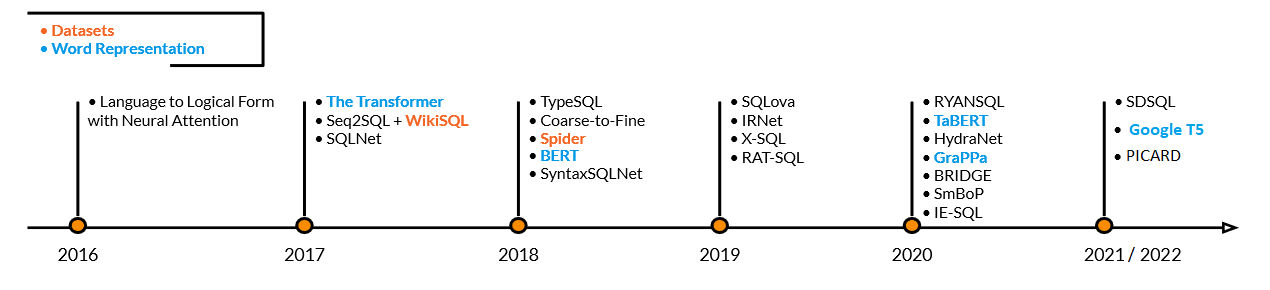
\includegraphics[width=0.99\textwidth]{pics/Timeline.png}
    \caption{Timeline of the deep learning process for Text-to-SQL.}
    \label{fig:timeline}
\end{figure}

This section will discuss existing cross-domain state-of-the-art (SOTA), text-to-SQL models, beginning with a broad overview and moving on to individual modules. This will provide a clear picture of the progress made in text-to-SQL research. Experiments have shown that pre-trained embeddings improve models because they construct better schema linking and a more accurate SQL structure.

An efficient text-to-SQL solution requires state-of-the-art natural language processing techniques.
As a result of the neural network's ability to handle only numerical inputs and not raw text, word embedding has been used to represent numerical words.
Aside from that, in the past few years, language models have become increasingly popular as a solution for increasing performance in natural language processing tasks.
Assuming that words have numerical representations that differ from those of other words, word embeddings aim to map each word to a multidimensional vector, incorporating valuable information about the word. In addition to the brute-force creation of one-hot embeddings, researchers have developed highly efficient methods for creating representations that convey a word's meaning and relationships with other words. In most, if not all, Text-to-SQL systems, word embedding techniques such as Word2Vec\cite{DBLP:journals/corr/Rong14}, and WordPiece embeddings\cite{DBLP:journals/corr/WuSCLNMKCGMKSJL16} are used.

Recently Language models have been shown to excel at NL tasks as a new type of pre-trained neural network. It is important to note that language models are not a replacement for word embeddings since they are neural networks and need a way to transform words into vectors.
Depending on the specific problem they want to solve, researchers can adapt the pre-trained model's inputs and outputs and train it for an additional number of epochs on their dataset. Thus, we can achieve state-of-the-art performance without complex architectures \cite{DBLP:journals/corr/abs-1810-04805}. Recent neural network architectures, like the Transformer\cite{DBLP:journals/corr/VaswaniSPUJGKP17}, have been used to achieve such performance by these models, which excel at handling NL and sequences of NL that are characterized by connections between words. Several language models have been used to handle the text-to-SQL task, including BERT \cite{DBLP:journals/corr/abs-1810-04805}. BERT is a pre-trained language model that has been shown to achieve state-of-the-art performance in a variety of NLP tasks. BERT is a Transformer-based model that uses a bidirectional encoder to learn the representation of a word based on the context in which it appears. BERT has been used in several text-to-SQL models, such as BRIDGE \cite{lin_bridging_2020} and RAT-SQL \cite{wang_rat-sql_2021}.

\subsection{Sequence-to-SQL}

\subsubsection{Seq2Seq}

The seq2seq model\cite{DBLP:journals/corr/SutskeverVL14} is a type of neural network architecture that has revolutionized the field of natural language processing. It generates meaningful sequences from input data, such as translating one language into another or summarizing text. The primary components of the seq2seq model are an encoder and decoder, which work together to learn how to map inputs onto outputs in a way that preserves their meaning.

The encoder takes raw input data and converts it into a series of numerical vectors known as embeddings. These embeddings represent each word or phrase in the input sequence with its unique vector representation so that it can be understood by the decoder for further processing. The decoder then uses these representations and other parameters like attention weights and recurrent layers to generate output sequences based on what was learned during training time from previous examples given by humans or machines alike.

Seq2Seq models can be trained using techniques such as supervised learning, which is trained on a dataset of input-output pairs, or unsupervised learning, where the model is trained to reconstruct the input sequence. Attention mechanisms, such as the attention mechanism used in the Transformer model, can also be incorporated into Seq2Seq models to improve their performance by allowing the decoder to focus selectively on certain parts of the input sequence.

Finally, once appropriately trained on large datasets containing millions of examples across multiple languages (or even within just one), this powerful tool can be used for tasks such as machine translation between two different languages; automatically generating summaries; question-answering systems; voice recognition software; among many others! Seq2Seq models have become increasingly popular due to their ability to quickly process large volumes of information while still maintaining accuracy and efficiency when compared to traditional methods like rule-based algorithms. However, one of the significant challenges of Seq2Seq models is the risk of generating irrelevant or nonsensical outputs, known as the "exposure bias" problem. Researchers have proposed various solutions to this problem, such as using beam search during decoding.

% image of seq2seq.png
\begin{figure}[ht]
    \centering
    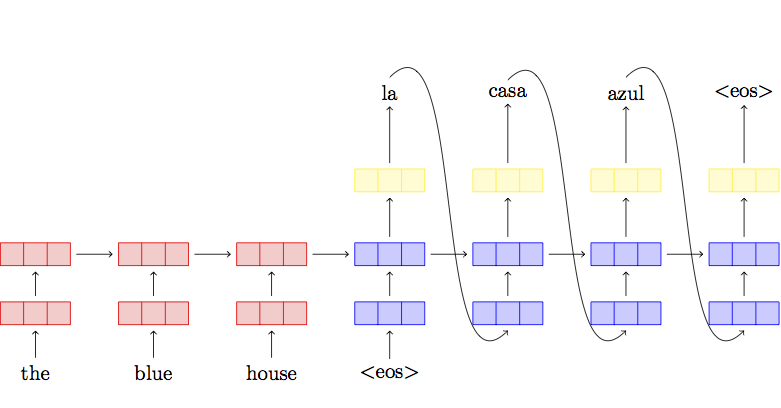
\includegraphics[width=0.5\textwidth]{pics/seq2seq.png}
    \caption{Example of Seq2Seq model in translating a sentence from English to French.\cite{DBLP:journals/corr/SutskeverVL14}}
    \label{fig:seq2seq}
\end{figure}

\subsubsection{Seq2SQL}

Seq2SQL \cite{zhong_seq2sql_2017} is a deep-learning system based on a straightforward concept: similar to Seq2Seq\cite{DBLP:journals/corr/SutskeverVL14}, it takes an input sentence or phrase, breaks it down into its components, and maps them onto a SQL query structure. Seq2SQL was one of the first deep-learning systems to employ this approach. However, later systems opted for different approaches due to the significant disadvantage of this approach: it does not consider the strict grammar rules of SQL when generating queries, making it the most error-prone. On the other hand, sequence-to-sequence architectures may have the potential to provide more accurate results but require more complex architectures to be implemented.

As part of this model, its authors released the WikiSQL dataset, which ushered in a new era of text-to-SQL deep learning research. With a seq-to-seq network, the system predicts the aggregation function and the column for the SELECT clause. Its major drawback is that it generates parts of the query that can lead to syntactic errors.
\subsection{SQLNet} \label{sec:sqlnet}

The model was designed to demonstrate that reinforcement learning should be limited to Text-to-SQL tasks.
Until SQLNet\cite{xu_sqlnet_2017}, all previous models used reinforcement learning to improve the decoder results when it generated appropriate serializations.


In cases where the order is irrelevant, SQLNet avoids the seq2seq structure.
For making predictions, the model uses a sketch-based approach consisting of a dependency graph that allows previous predictions to be taken into account.
The model also incorporates column attention (weights assigned to significant words and phrases in sentences) to improve the results. According to the flowchart below, SQLNet employs three phases to generate SQL queries for WikiSQL tasks.

% add image sqlnet.png
% \begin{figure}[H]
%     \centering
%     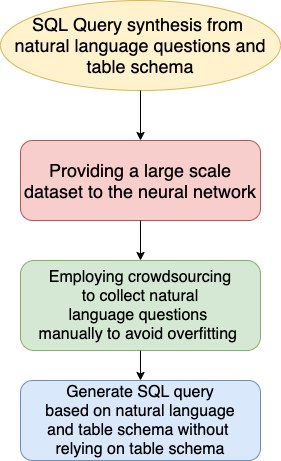
\includegraphics[width=0.3\textwidth]{pics/sqlnet/sqlnet.png}
%     \caption{SQLNet\cite{xu_sqlnet_2017}}
%     \label{fig:sqlnet}
% \end{figure}

\subsubsection*{Sketch-based query synthesis}

The token with the \$ sign represents an empty slot, and the token name represents the type of prediction. Tokens in bold represent SQL keywords such as SELECT, WHERE, etc.
\$AGG can be filled with either an empty token or one of the aggregation operators, such as SUM or MAX. Fill in the \$COLUMN and \$VALUE slots with the column name and substring of the question, respectively. The \$OP slot can be a value between \{=, \}. The notion \(...\)* uses a regular expression to indicate zero or more AND clauses.

\begin{figure}[H]
    \centering
    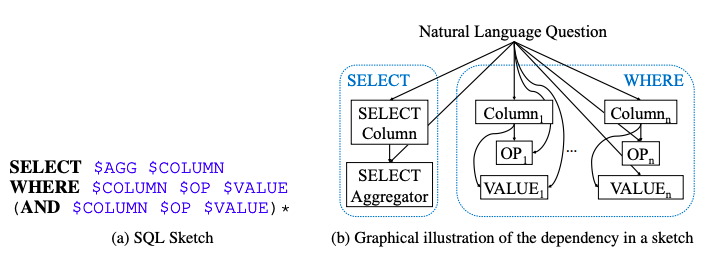
\includegraphics[width=0.8\textwidth]{pics/sqlnet/sketch-based.png}
    \caption{Sketch-based query synthesis\cite{xu_sqlnet_2017}}
    \label{fig:sketch-based}
\end{figure}

% bold text
\subsubsection*{Column attention for sequence-to-set prediction}

Instead of producing a sequence of column names, sequence-to-set prediction predicts the names of the columns of interest.
Based on column names, column attention is part of the generic attention mechanism for computing the feature attention map on a question.

\subsubsection*{Predicting WHERE and SELECT clause}

One of the most challenging tasks in Text-to-SQL is predicting the WHERE clause.
According to SQL sketch, SQLNet finds the columns that appear in the WHERE clause and predicts the OP slots and value for each column.

It is predicted that the OP slot will be filled with one of the three classes \{<,>,=\}, and the VALUE slot will be filled with the substring from the natural language question.
In SELECT clauses, columns are named, and aggregator functions are specified, such as count, sum, max, etc. There is only one difference between SELECT and WHERE: the column name. There is only one column selected in SELECT.

In the WikiSQL test set, SQLNet accuracy is 64.4\%, and in the SPIDER test set, it is around 12.4\%.

\begin{figure}[H]
    \centering
    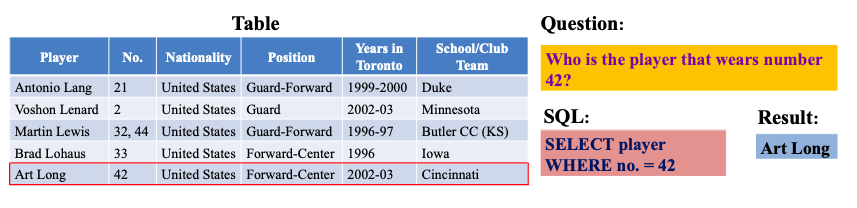
\includegraphics[width=0.8\textwidth]{pics/sqlnet/sqlnet-task.png}
    \caption{An example of a query executed by SQLNet on WikiSQL\cite{xu_sqlnet_2017}}
    \label{fig:sqlnet-task}
\end{figure}
\subsection{SyntaxSQLNet}

The main\cite{DBLP:journals/corr/abs-1810-05237} goal of developing the SyntaxSQLNet model was to generate complex SQL queries with multiple clauses and generalize them to new databases.
This was achieved through the use of a syntax tree network, which is capable of addressing complex and cross-domain queries.
As is evident in the chart below, the SyntaxSQLNet model is composed of several components, each with its unique function and purpose in generating complex SQL queries. The encoders are table-aware, while the decoders have a history of the SQL generation path.

With a massive 7.3\% improvement in accuracy, SyntaxSQLNet outperformed previous models, such as SQLNet, on the SPIDER dataset.
A cross-domain data augmentation technique was employed to improve accuracy further to generate more variance during training, allowing for a greater degree of accuracy and robustness.

\begin{figure}[htb]
    \centering
    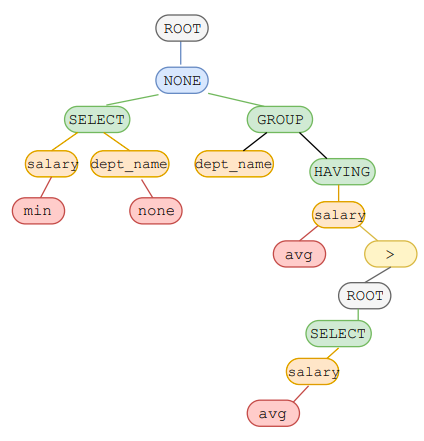
\includegraphics[width=0.6\textwidth]{pics/SyntaxSQLNet/Tree-based.png}
    \caption{Tree-based SQL generator in SyntaxSQLNet\cite{DBLP:journals/corr/abs-1810-05237}}
    \label{fig:tree-based}
\end{figure}

\begin{figure}[htb]
    \centering
    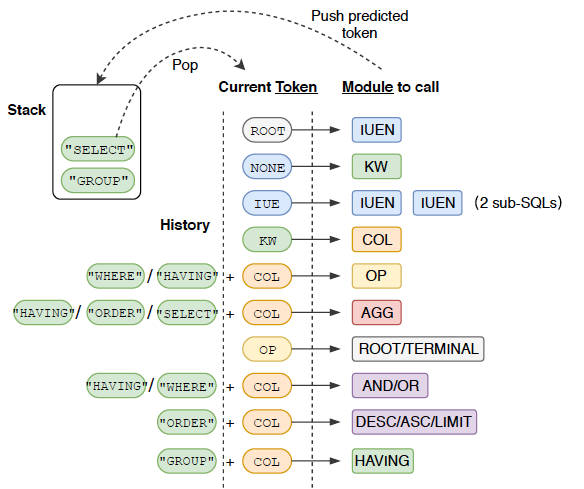
\includegraphics[width=0.8\textwidth]{pics/SyntaxSQLNet/Grammar.png}
    \caption{Modules defined in SyntaxSQLNet model\cite{DBLP:journals/corr/abs-1810-05237}}
    \label{fig:grammar}
\end{figure}

\subsubsection*{SQL Grammar and Attention Mechanism}

To enable the decoder to handle complex queries, SQL grammar is employed in order to allow the decoder to make decisions at each step of recursive decoding. This allows the decoder to determine which module to invoke for the prediction of the following SQL token, taking into account the history of SQL path generation, the current SQL tokens, and the attention mechanism. The attention mechanism is used to encode the question representation, which is then applied to the SQL path history encoding. This is advantageous as it allows for a more detailed representation of the query to be created, which in turn leads to more efficient and accurate responses.

\subsubsection*{Data Augmentation}

Despite SPIDER's large dataset, it lacks complex queries. To achieve proper generalization, cross-domain datasets are used for data augmentation. The SPIDER dataset is used to prepare a list of patterns for natural language questions and corresponding SQL queries. The SPIDER model, using syntaxSQLNet decoding history, reaches 27.2\% accuracy, an increase of 12.4\% compared to previous models such as SQLNet.
\subsubsection{TypeSQL 2018}

TypeSQL, proposed by Yu et al. (2018), is an enhanced version of SQLNet. It introduces a new training process and uses types obtained from knowledge graphs or table content to help the model better understand the entities and numbers in question. This process helps the model comprehend the semantics of the query and effectively use the context information of the database. In our experiment, we extracted question type info from database content and extended the modules to include ORDER BY and GROUP BY components. This makes TypeSQL the only model incorporating database content, providing a more complete and accurate understanding of the query. With these enhanced features, TypeSQL can better understand the query and produce more accurate results.

% direct copy
In contrast, SQLNet and TypeSQL that utilize SQL structure information to guide the SQL generation process significantly outperform other Seq2Seq models. While they can produce valid queries, however, they are unable to generate nested queries or queries with keywords such as EXCEPT and INTERSECT because they limit possible SQL outputs in some fixed pre-defined SQL structures.
\subsection{IRNet 2019}
IRNET \cite{DBLP:journals/corr/abs-1905-08205}

\begin{itemize}
    \item In Text2SQL tasks, the Intermediate Representation Network (IRNet) addresses two main challenges.
    \item Among the challenges are mismatches between natural language intents and predicting columns resulting from a more significant number of out-of-domain words.
    \item Instead of synthesizing SQL queries end-to-end, IRNet decomposes natural language into three phases.
    \item Schema linking is performed over a database schema and a question during the first phase.
    \item IRNet uses SemQL to bridge the gap between SQL and natural language.
    \item It includes a Natural Language (NL) encoder, a Schema Encoder, and a Decoder.
\end{itemize}

\begin{figure}[htb]
    \centering
    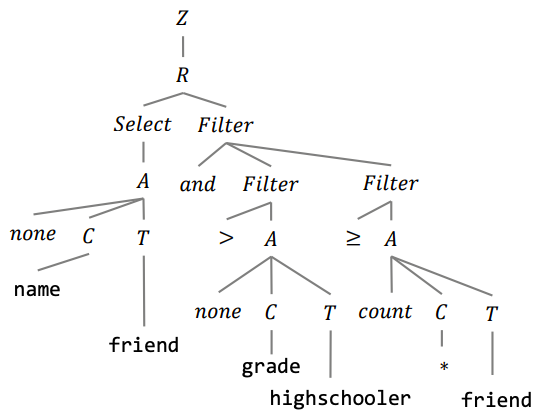
\includegraphics[width=0.5\textwidth]{pics/IRNet/illustrative_SemSQL}
    \caption{An illustrative example of SemSQL from \cite{DBLP:journals/corr/abs-1905-08205}}
    \label{fig:illustrative_SemSQL}
\end{figure}

\begin{figure}[htb]
    \centering
    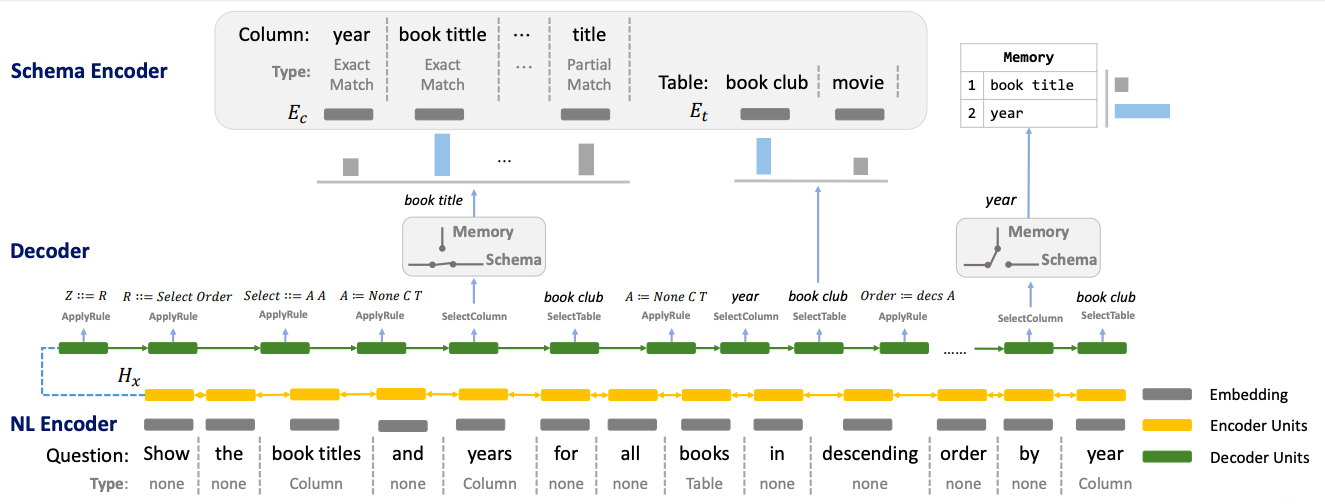
\includegraphics[width=0.8\textwidth]{pics/IRNet/overview}
    \caption{An overview of the neural model proposed in \cite{DBLP:journals/corr/abs-1905-08205}}
    \label{fig:overview}
\end{figure}

\begin{itemize}
    \item The model provides different functions to accomplish Text2SQL tasks.
    \item Natural language is encoded into an embedding vector by the NL encoder. By using a bi-directional LSTM, these embedding vectors are used to construct hidden states.
    \item A schema encoder takes a database schema as input and outputs representations for columns and tables.
    \item Using context-free grammar, the decoder synthesizes SemQL queries.
    \item On the SPIDER dataset, IRNet performs 46.7\% better than previous benchmark models by 19%.
    \item The accuracy of 54.7\% is achieved by combining IRNet with BERT.
\end{itemize}

\begin{figure}[htb]
    \centering
    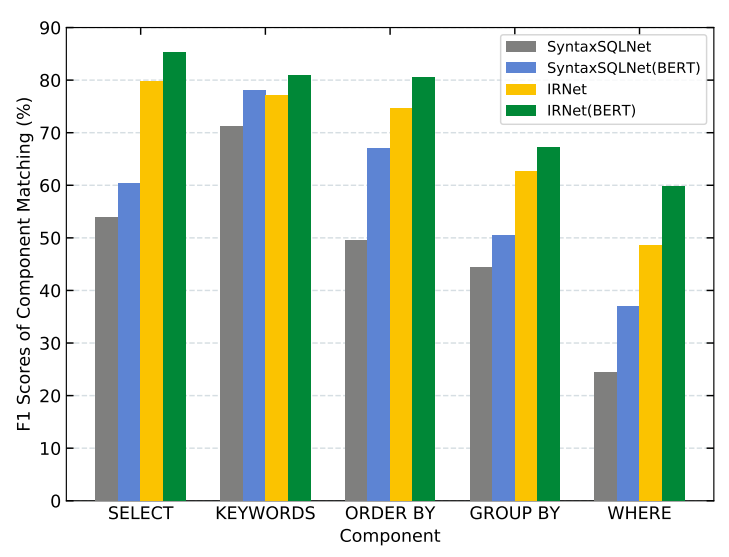
\includegraphics[width=0.6\textwidth]{pics/IRNet/f1}
    \caption{F1 scores of component matching of SyntaxSQLNet, SyntaxSQLNet\(BERT\), IRNet and IRNet\(BERT\) on the test set from \cite{DBLP:journals/corr/abs-1905-08205}}
    \label{fig:f1}
\end{figure}

\subsection{EditSQL}

EditSQL\cite{DBLP:journals/corr/abs-1909-00786} focuses on text-to-SQL tasks that are context-dependent across domains.
It exploits the fact that adjacent natural language questions are dependent on one another and that corresponding SQL queries overlap.
To improve the generation quality, they edit the previously predicted query.
The editing mechanism reuses generation results at the token level based on SQL input sequences.
An utterance-table encoder and a table-aware decoder are utilized to incorporate the context of the natural language and the schema when dealing with complicated tables in different domains.

\begin{figure}[htb]
    \centering
    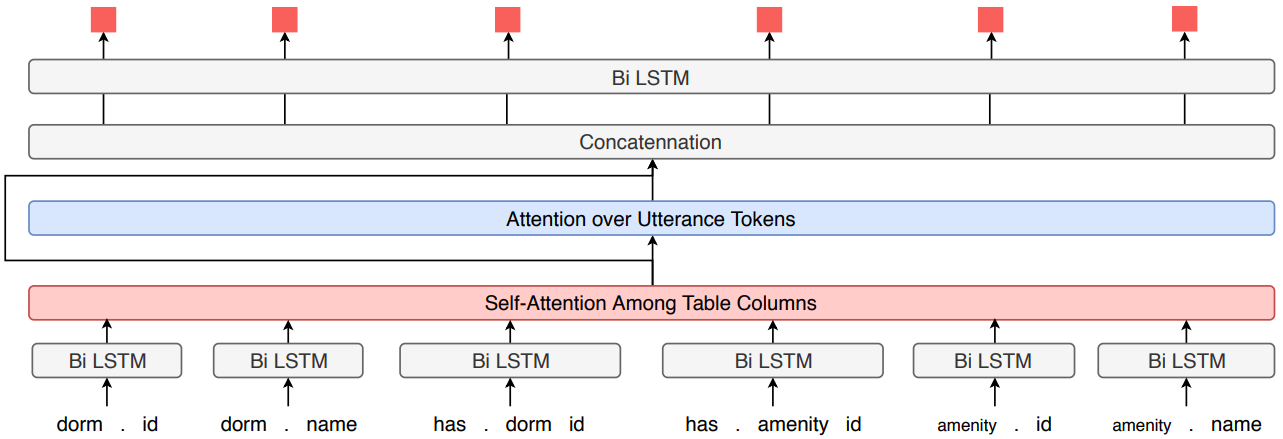
\includegraphics[width=0.8\textwidth]{pics/EditSQL/Table.png}
    \caption{The model architecture of EditSQL \cite{DBLP:journals/corr/abs-1909-00786}}
    \label{fig:EditSQL}
\end{figure}

User utterances and table schemas are encoded by the utterance-table encoder. Tokens of utterances are encoded using a bi-LSTM.
To determine the most relevant columns, Attention weighed an average of column header embedding is applied to each token.

\begin{figure}[htb]
    \centering
    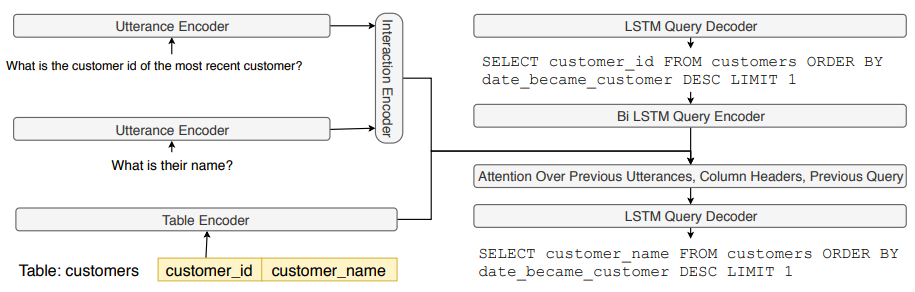
\includegraphics[width=0.9\textwidth]{pics/EditSQL/model.png}
    \caption{An example of user utterance and column headers and Utterance Encoder \cite{DBLP:journals/corr/abs-1909-00786}}
    \label{fig:EditSQL_model}
\end{figure}

To capture the relationship between table schema and utterance, an attention layer is incorporated.
The utterance-level encoder is built on top of an interaction-level decoder in order to capture information across utterances.
LSTM decoding is used to generate SQL queries by incorporating interaction history, table schema, and user utterances.

\begin{figure}[htb]
    \centering
    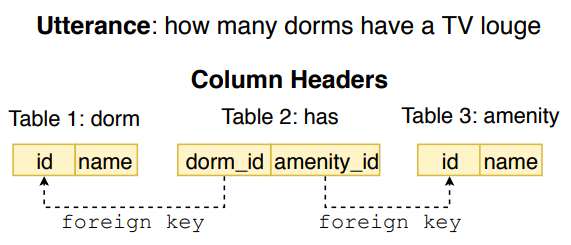
\includegraphics[width=0.5\textwidth]{pics/EditSQL/example.png}
    \caption{Table Encoder \cite{DBLP:journals/corr/abs-1909-00786}}
    \label{fig:EditSQL_example}
\end{figure}

The SPIDER dataset was used to evaluate the model, which outperformed the previous state-of-the-art model, such as IRNet. The model achieved a 32.9\% accuracy, and by using BERT embedding, a 57.9\% improvement in accuracy was achieved.
\subsection*{RAT-SQL}

\begin{figure}[htb]
    \centering
    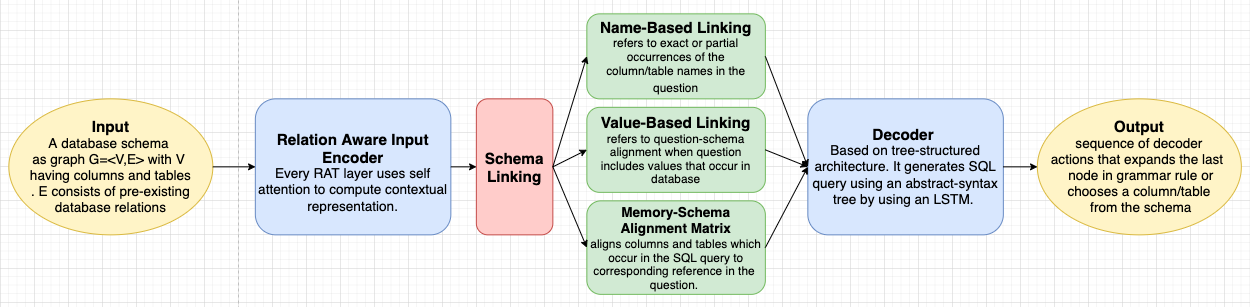
\includegraphics[width=0.8\textwidth]{pics/RAT-SQL/flow.png}
    \caption{A flow chart of RAT-SQL model}
    \label{fig:RAT-SQL-flow}
\end{figure}

\begin{itemize}
    \item A major challenge in translating natural language queries into SQL queries is generalizing them to unknown database schemas.
    \item As part of the generalisation, it is necessary to encode database relations in an accessible way and model alignment between relevant database columns in the query.
    \item Within a text2SQL encoder, the proposed framework leverages the relation-aware self-attention mechanism to encode address schemas, represent features, and link schemas.
    \item Check out the flow chart below for an overview of RAT-SQL's encoder-decoder structure.
\end{itemize}

\begin{figure}[htb]
    \centering
    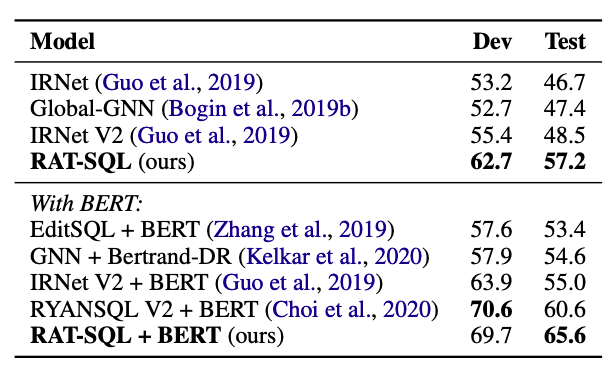
\includegraphics[width=0.4\textwidth]{pics/RAT-SQL/Accuracy.png}
    \caption{Accuracy on the Spider development and test sets, compared to the other approaches at the top of the dataset leaderboard as of May 1st, 2020 from \cite{wang_rat-sql_2021}}
    \label{fig:RAT-SQL-Accuracy}
\end{figure}

On the SPIDER dataset, RAT-SQL achieves 57.2\% accuracy, an improvement of 8.7\% over previous benchmark models.

\begin{figure}[htb]
    \centering
    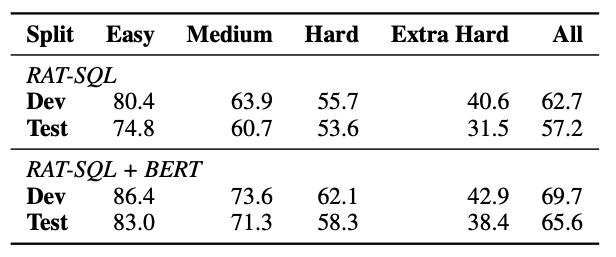
\includegraphics[width=0.4\textwidth]{pics/RAT-SQL/Accuracy2.png}
    \caption{Accuracy on the Spider development and test sets, by difficulty from \cite{wang_rat-sql_2021}}
    \label{fig:RAT-SQL-Accuracy2}
\end{figure}

With RAT-SQL, 65.6\% accuracy can be achieved by combining BERT with RAT-SQL.

% \input{inc/models/BRIDGE}
\subsection*{Picard}

Picard\cite{scholak_picard_2021} stands for "Parsing Incrementally for Constrained Auto-Regressive Decoding.". It can be used with any existing language model decoder or vocabulary based on auto-regressive language modeling.

As an optional feature, Picard can be enabled at inference time and is absent from pre-training or fine-tuning. In the case of text-to-SQL translation, Picard operates directly on the output of the language model.
Picard demonstrates state-of-the-art performance on challenging Spider and CoSQL text-to-SQL translation tasks.

Picard warps model prediction scores and integrates trivially with existing greedy and beam search algorithms. In addition to the token ids of the current hypothesis, the model's language modeling head also predicts the log-softmax scores for each vocabulary token. Additionally, Picard has access to SQL schema information, including table and column names and which column resides in which table.
\subsection{RASAT}

RASAT \cite{https://doi.org/10.48550/arxiv.2205.06983}